% !TeX program = xelatex
% !TeX encoding = UTF-8

\documentclass[11pt,a4paper]{article}

% 中文支持（保留以便支持中英混合内容）
\usepackage[UTF8]{ctex}

% Page setup
\usepackage[left=2cm,right=2cm,top=2cm,bottom=2cm]{geometry}
\usepackage{ragged2e}
\usepackage[none]{hyphenat}

% Graphics support
\usepackage{graphicx}
\usepackage{tikz}

% Fonts and colors
\usepackage{xcolor}
\usepackage{fontawesome5}

% Define theme colors
\definecolor{primarycolor}{RGB}{41, 128, 185}
\definecolor{secondarycolor}{RGB}{52, 73, 94}
\definecolor{accentcolor}{RGB}{231, 76, 60}
\definecolor{decorcolor}{RGB}{230, 126, 34}

% Set paragraph spacing
\setlength{\parskip}{0.15em}

\usepackage{titlesec}
\titlespacing{\section}{0pt}{8pt}{5pt}

% List formatting
\usepackage{enumitem}
\setlist[itemize]{leftmargin=1.2em,topsep=0.1em,itemsep=0.05em}

\begin{document}

% Header section
\vspace{-0.2cm}
\begin{minipage}[t]{0.75\textwidth}
    \vspace{0.3cm}
    {\Huge \bfseries \color{secondarycolor} Zhang San}

    \vspace{0.15cm}

    {\large Software Engineer}

    \vspace{0.25cm}

    % Contact information
    \color{secondarycolor}
    {\faPhone} +86 138-xxxx-xxxx \hspace{0.6cm}
    {\faEnvelope} zhangsan@email.com \hspace{0.6cm}
    {\faMapMarker} Beijing, China

    \vspace{0.1cm}

    {\faWeixin} zhangsan\_wx \hspace{0.6cm}
    {\faGithub} github.com/zhangsan
\end{minipage}%
\hfill
\begin{minipage}[t]{0.2\textwidth}
    \vspace{0.3cm}
    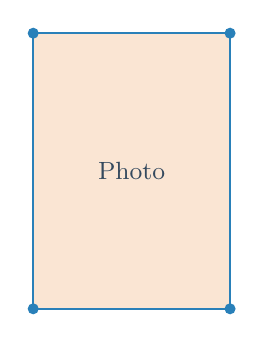
\begin{tikzpicture}
        % One-inch photo frame decoration
        \fill[decorcolor!20] (0,0) rectangle (2.5,3.5);
        \draw[primarycolor,thick] (0,0) rectangle (2.5,3.5);
        % Corner decorations
        \foreach \x/\y in {0/0,0/3.5,2.5/0,2.5/3.5}
            \fill[primarycolor] (\x,\y) circle (2pt);
        \node[text width=2cm,align=center,font=\small\color{secondarycolor}] at (1.25,1.75) {Photo};
        % Uncomment the following line to add your photo
        % \node[anchor=south west,inner sep=0] at (0,0) {\includegraphics[width=2.5cm,height=3.5cm]{photo.jpg}};
    \end{tikzpicture}
\end{minipage}

\vspace{0.3cm}

% Education
\section*{\faGraduationCap\quad Education}

\begin{itemize}
    \item \textbf{Master of Computer Science and Technology} \hfill Sep 2016 -- Jan 2019

    \textcolor{primarycolor}{Tsinghua University}

    \vspace{0.05em}

    Core Courses: Advanced Algorithms, Distributed Systems, Machine Learning, Database Systems, Software Engineering

    \vspace{0.15em}

    \item \textbf{Bachelor of Software Engineering} \hfill Sep 2012 -- Jun 2016

    \textcolor{primarycolor}{Zhejiang University}

    \vspace{0.05em}

    GPA: 3.8/4.0, University Scholarship for Three Consecutive Years
\end{itemize}

\section*{\faBriefcase\quad Internship/Project Experience}

\begin{itemize}
    \item \textbf{Senior Software Engineer} \hfill Jun 2021 -- Present

    \textcolor{primarycolor}{Beijing Technology Co., Ltd.}

    \begin{itemize}
        \item Responsible for architecture design and development of the company's core SaaS platform, with over 1 million users
        \item Led the migration from monolithic architecture to microservices, improving system response time by 60\%
        \item Managed a 5-person development team, completed multiple key version iterations with 95\% on-time delivery rate
        \item Introduced CI/CD pipeline, reducing code deployment time from 2 hours to 15 minutes
    \end{itemize}

    \vspace{0.15em}

    \item \textbf{Software Engineer} \hfill Mar 2019 -- May 2021

    \textcolor{primarycolor}{Shanghai Internet Company}

    \begin{itemize}
        \item Participated in development of e-commerce order and payment systems, processing 500k+ orders daily
        \item Optimized database query performance, reducing core API response time from 500ms to 100ms
        \item Designed and implemented a message queue system, effectively solving message loss in high-concurrency scenarios
    \end{itemize}

    \vspace{0.15em}

    \item \textbf{Enterprise Data Analytics Platform} \hfill Jan 2023 -- Aug 2023

    \textcolor{primarycolor}{Personal Project}

    \begin{itemize}
        \item Built a real-time data analytics system using React + Spring Boot + Kafka
        \item Designed and implemented visualization reporting features with custom report export
        \item System supports 10+ TB of data processing with query response time < 3 seconds
    \end{itemize}

    \vspace{0.15em}

    \item \textbf{Intelligent Customer Service System} \hfill Mar 2022 -- Oct 2022

    \textcolor{primarycolor}{Personal Project}

    \begin{itemize}
        \item Built an intelligent Q\&A chatbot based on NLP technology, resolving 80\% of common user inquiries
        \item Designed session management module supporting multi-turn conversations and context understanding
        \item Integrated with WeChat and DingTalk platforms, serving over 500k users
    \end{itemize}
\end{itemize}

\section*{\faTools\quad IT Skills}

\begin{itemize}
    \item \textbf{Programming Languages}: Java, Python, JavaScript/TypeScript, Go, SQL
    \item \textbf{Frontend}: React, Vue.js, HTML5/CSS3, Node.js
    \item \textbf{Backend Frameworks}: Spring Boot, Django, Flask, gRPC
    \item \textbf{Databases}: MySQL, PostgreSQL, MongoDB, Redis
    \item \textbf{Cloud Services}: AWS, Alibaba Cloud, Docker, Kubernetes
    \item \textbf{Development Tools}: Git, Jenkins, VS Code, IntelliJ IDEA
\end{itemize}

\section*{\faAward\quad Awards \& Certifications}

\begin{itemize}
    \item \textbf{Outstanding Employee Award 2022} \hfill Beijing Technology Co., Ltd.
    \item \textbf{PMP Project Management Certification} \hfill PMI Certified
    \item \textbf{AWS Certified Solutions Architect} \hfill Amazon Web Services
    \item \textbf{Silver Award, National College Student Innovation Competition} \hfill 2015
\end{itemize}

\section*{\faInfoCircle\quad Additional Information}

\begin{itemize}
    \item \textbf{Language}: CET-6 (520), able to read English technical documents fluently
    \item \textbf{Interests}: Photography, Marathon, Open Source Community Contribution
    \item \textbf{Self-evaluation}: Passionate about technology, continuous learner, good at communication and collaboration
\end{itemize}

\end{document}
